\documentclass{article} % For LaTeX2e
\usepackage{iclr2021_conference,times}

% Optional math commands from https://github.com/goodfeli/dlbook_notation.
% DO NOT MODIFY THIS COMMENT
% read `https://github.com/James-Yu/LaTeX-Workshop/wiki/Compile#the-root-file`
% read `https://github.com/James-Yu/LaTeX-Workshop/issues/1165`
% !TEX root = iclr2021_conference.tex

%%%%% NEW MATH DEFINITIONS %%%%%

\usepackage{amsmath,amsfonts,bm}

% Mark sections of captions for referring to divisions of figures
\newcommand{\figleft}{{\em (Left)}}
\newcommand{\figcenter}{{\em (Center)}}
\newcommand{\figright}{{\em (Right)}}
\newcommand{\figtop}{{\em (Top)}}
\newcommand{\figbottom}{{\em (Bottom)}}
\newcommand{\captiona}{{\em (a)}}
\newcommand{\captionb}{{\em (b)}}
\newcommand{\captionc}{{\em (c)}}
\newcommand{\captiond}{{\em (d)}}

% Highlight a newly defined term
\newcommand{\newterm}[1]{{\bf #1}}


% Figure reference, lower-case.
\def\figref#1{figure~\ref{#1}}
% Figure reference, capital. For start of sentence
\def\Figref#1{Figure~\ref{#1}}
\def\twofigref#1#2{figures \ref{#1} and \ref{#2}}
\def\quadfigref#1#2#3#4{figures \ref{#1}, \ref{#2}, \ref{#3} and \ref{#4}}
% Section reference, lower-case.
\def\secref#1{section~\ref{#1}}
% Section reference, capital.
\def\Secref#1{Section~\ref{#1}}
% Reference to two sections.
\def\twosecrefs#1#2{sections \ref{#1} and \ref{#2}}
% Reference to three sections.
\def\secrefs#1#2#3{sections \ref{#1}, \ref{#2} and \ref{#3}}
% Reference to an equation, lower-case.
\def\eqref#1{equation~\ref{#1}}
% Reference to an equation, upper case
\def\Eqref#1{Equation~\ref{#1}}
% A raw reference to an equation---avoid using if possible
\def\plaineqref#1{\ref{#1}}
% Reference to a chapter, lower-case.
\def\chapref#1{chapter~\ref{#1}}
% Reference to an equation, upper case.
\def\Chapref#1{Chapter~\ref{#1}}
% Reference to a range of chapters
\def\rangechapref#1#2{chapters\ref{#1}--\ref{#2}}
% Reference to an algorithm, lower-case.
\def\algref#1{algorithm~\ref{#1}}
% Reference to an algorithm, upper case.
\def\Algref#1{Algorithm~\ref{#1}}
\def\twoalgref#1#2{algorithms \ref{#1} and \ref{#2}}
\def\Twoalgref#1#2{Algorithms \ref{#1} and \ref{#2}}
% Reference to a part, lower case
\def\partref#1{part~\ref{#1}}
% Reference to a part, upper case
\def\Partref#1{Part~\ref{#1}}
\def\twopartref#1#2{parts \ref{#1} and \ref{#2}}

\def\ceil#1{\lceil #1 \rceil}
\def\floor#1{\lfloor #1 \rfloor}
\def\1{\bm{1}}
\newcommand{\train}{\mathcal{D}}
\newcommand{\valid}{\mathcal{D_{\mathrm{valid}}}}
\newcommand{\test}{\mathcal{D_{\mathrm{test}}}}

\def\eps{{\epsilon}}


% Random variables
\def\reta{{\textnormal{$\eta$}}}
\def\ra{{\textnormal{a}}}
\def\rb{{\textnormal{b}}}
\def\rc{{\textnormal{c}}}
\def\rd{{\textnormal{d}}}
\def\re{{\textnormal{e}}}
\def\rf{{\textnormal{f}}}
\def\rg{{\textnormal{g}}}
\def\rh{{\textnormal{h}}}
\def\ri{{\textnormal{i}}}
\def\rj{{\textnormal{j}}}
\def\rk{{\textnormal{k}}}
\def\rl{{\textnormal{l}}}
% rm is already a command, just don't name any random variables m
\def\rn{{\textnormal{n}}}
\def\ro{{\textnormal{o}}}
\def\rp{{\textnormal{p}}}
\def\rq{{\textnormal{q}}}
\def\rr{{\textnormal{r}}}
\def\rs{{\textnormal{s}}}
\def\rt{{\textnormal{t}}}
\def\ru{{\textnormal{u}}}
\def\rv{{\textnormal{v}}}
\def\rw{{\textnormal{w}}}
\def\rx{{\textnormal{x}}}
\def\ry{{\textnormal{y}}}
\def\rz{{\textnormal{z}}}

% Random vectors
\def\rvepsilon{{\mathbf{\epsilon}}}
\def\rvtheta{{\mathbf{\theta}}}
\def\rva{{\mathbf{a}}}
\def\rvb{{\mathbf{b}}}
\def\rvc{{\mathbf{c}}}
\def\rvd{{\mathbf{d}}}
\def\rve{{\mathbf{e}}}
\def\rvf{{\mathbf{f}}}
\def\rvg{{\mathbf{g}}}
\def\rvh{{\mathbf{h}}}
\def\rvu{{\mathbf{i}}}
\def\rvj{{\mathbf{j}}}
\def\rvk{{\mathbf{k}}}
\def\rvl{{\mathbf{l}}}
\def\rvm{{\mathbf{m}}}
\def\rvn{{\mathbf{n}}}
\def\rvo{{\mathbf{o}}}
\def\rvp{{\mathbf{p}}}
\def\rvq{{\mathbf{q}}}
\def\rvr{{\mathbf{r}}}
\def\rvs{{\mathbf{s}}}
\def\rvt{{\mathbf{t}}}
\def\rvu{{\mathbf{u}}}
\def\rvv{{\mathbf{v}}}
\def\rvw{{\mathbf{w}}}
\def\rvx{{\mathbf{x}}}
\def\rvy{{\mathbf{y}}}
\def\rvz{{\mathbf{z}}}

% Elements of random vectors
\def\erva{{\textnormal{a}}}
\def\ervb{{\textnormal{b}}}
\def\ervc{{\textnormal{c}}}
\def\ervd{{\textnormal{d}}}
\def\erve{{\textnormal{e}}}
\def\ervf{{\textnormal{f}}}
\def\ervg{{\textnormal{g}}}
\def\ervh{{\textnormal{h}}}
\def\ervi{{\textnormal{i}}}
\def\ervj{{\textnormal{j}}}
\def\ervk{{\textnormal{k}}}
\def\ervl{{\textnormal{l}}}
\def\ervm{{\textnormal{m}}}
\def\ervn{{\textnormal{n}}}
\def\ervo{{\textnormal{o}}}
\def\ervp{{\textnormal{p}}}
\def\ervq{{\textnormal{q}}}
\def\ervr{{\textnormal{r}}}
\def\ervs{{\textnormal{s}}}
\def\ervt{{\textnormal{t}}}
\def\ervu{{\textnormal{u}}}
\def\ervv{{\textnormal{v}}}
\def\ervw{{\textnormal{w}}}
\def\ervx{{\textnormal{x}}}
\def\ervy{{\textnormal{y}}}
\def\ervz{{\textnormal{z}}}

% Random matrices
\def\rmA{{\mathbf{A}}}
\def\rmB{{\mathbf{B}}}
\def\rmC{{\mathbf{C}}}
\def\rmD{{\mathbf{D}}}
\def\rmE{{\mathbf{E}}}
\def\rmF{{\mathbf{F}}}
\def\rmG{{\mathbf{G}}}
\def\rmH{{\mathbf{H}}}
\def\rmI{{\mathbf{I}}}
\def\rmJ{{\mathbf{J}}}
\def\rmK{{\mathbf{K}}}
\def\rmL{{\mathbf{L}}}
\def\rmM{{\mathbf{M}}}
\def\rmN{{\mathbf{N}}}
\def\rmO{{\mathbf{O}}}
\def\rmP{{\mathbf{P}}}
\def\rmQ{{\mathbf{Q}}}
\def\rmR{{\mathbf{R}}}
\def\rmS{{\mathbf{S}}}
\def\rmT{{\mathbf{T}}}
\def\rmU{{\mathbf{U}}}
\def\rmV{{\mathbf{V}}}
\def\rmW{{\mathbf{W}}}
\def\rmX{{\mathbf{X}}}
\def\rmY{{\mathbf{Y}}}
\def\rmZ{{\mathbf{Z}}}

% Elements of random matrices
\def\ermA{{\textnormal{A}}}
\def\ermB{{\textnormal{B}}}
\def\ermC{{\textnormal{C}}}
\def\ermD{{\textnormal{D}}}
\def\ermE{{\textnormal{E}}}
\def\ermF{{\textnormal{F}}}
\def\ermG{{\textnormal{G}}}
\def\ermH{{\textnormal{H}}}
\def\ermI{{\textnormal{I}}}
\def\ermJ{{\textnormal{J}}}
\def\ermK{{\textnormal{K}}}
\def\ermL{{\textnormal{L}}}
\def\ermM{{\textnormal{M}}}
\def\ermN{{\textnormal{N}}}
\def\ermO{{\textnormal{O}}}
\def\ermP{{\textnormal{P}}}
\def\ermQ{{\textnormal{Q}}}
\def\ermR{{\textnormal{R}}}
\def\ermS{{\textnormal{S}}}
\def\ermT{{\textnormal{T}}}
\def\ermU{{\textnormal{U}}}
\def\ermV{{\textnormal{V}}}
\def\ermW{{\textnormal{W}}}
\def\ermX{{\textnormal{X}}}
\def\ermY{{\textnormal{Y}}}
\def\ermZ{{\textnormal{Z}}}

% Vectors
\def\vzero{{\bm{0}}}
\def\vone{{\bm{1}}}
\def\vmu{{\bm{\mu}}}
\def\vtheta{{\bm{\theta}}}
\def\va{{\bm{a}}}
\def\vb{{\bm{b}}}
\def\vc{{\bm{c}}}
\def\vd{{\bm{d}}}
\def\ve{{\bm{e}}}
\def\vf{{\bm{f}}}
\def\vg{{\bm{g}}}
\def\vh{{\bm{h}}}
\def\vi{{\bm{i}}}
\def\vj{{\bm{j}}}
\def\vk{{\bm{k}}}
\def\vl{{\bm{l}}}
\def\vm{{\bm{m}}}
\def\vn{{\bm{n}}}
\def\vo{{\bm{o}}}
\def\vp{{\bm{p}}}
\def\vq{{\bm{q}}}
\def\vr{{\bm{r}}}
\def\vs{{\bm{s}}}
\def\vt{{\bm{t}}}
\def\vu{{\bm{u}}}
\def\vv{{\bm{v}}}
\def\vw{{\bm{w}}}
\def\vx{{\bm{x}}}
\def\vy{{\bm{y}}}
\def\vz{{\bm{z}}}

% Elements of vectors
\def\evalpha{{\alpha}}
\def\evbeta{{\beta}}
\def\evepsilon{{\epsilon}}
\def\evlambda{{\lambda}}
\def\evomega{{\omega}}
\def\evmu{{\mu}}
\def\evpsi{{\psi}}
\def\evsigma{{\sigma}}
\def\evtheta{{\theta}}
\def\eva{{a}}
\def\evb{{b}}
\def\evc{{c}}
\def\evd{{d}}
\def\eve{{e}}
\def\evf{{f}}
\def\evg{{g}}
\def\evh{{h}}
\def\evi{{i}}
\def\evj{{j}}
\def\evk{{k}}
\def\evl{{l}}
\def\evm{{m}}
\def\evn{{n}}
\def\evo{{o}}
\def\evp{{p}}
\def\evq{{q}}
\def\evr{{r}}
\def\evs{{s}}
\def\evt{{t}}
\def\evu{{u}}
\def\evv{{v}}
\def\evw{{w}}
\def\evx{{x}}
\def\evy{{y}}
\def\evz{{z}}

% Matrix
\def\mA{{\bm{A}}}
\def\mB{{\bm{B}}}
\def\mC{{\bm{C}}}
\def\mD{{\bm{D}}}
\def\mE{{\bm{E}}}
\def\mF{{\bm{F}}}
\def\mG{{\bm{G}}}
\def\mH{{\bm{H}}}
\def\mI{{\bm{I}}}
\def\mJ{{\bm{J}}}
\def\mK{{\bm{K}}}
\def\mL{{\bm{L}}}
\def\mM{{\bm{M}}}
\def\mN{{\bm{N}}}
\def\mO{{\bm{O}}}
\def\mP{{\bm{P}}}
\def\mQ{{\bm{Q}}}
\def\mR{{\bm{R}}}
\def\mS{{\bm{S}}}
\def\mT{{\bm{T}}}
\def\mU{{\bm{U}}}
\def\mV{{\bm{V}}}
\def\mW{{\bm{W}}}
\def\mX{{\bm{X}}}
\def\mY{{\bm{Y}}}
\def\mZ{{\bm{Z}}}
\def\mBeta{{\bm{\beta}}}
\def\mPhi{{\bm{\Phi}}}
\def\mLambda{{\bm{\Lambda}}}
\def\mSigma{{\bm{\Sigma}}}

% Tensor
\DeclareMathAlphabet{\mathsfit}{\encodingdefault}{\sfdefault}{m}{sl}
\SetMathAlphabet{\mathsfit}{bold}{\encodingdefault}{\sfdefault}{bx}{n}
\newcommand{\tens}[1]{\bm{\mathsfit{#1}}}
\def\tA{{\tens{A}}}
\def\tB{{\tens{B}}}
\def\tC{{\tens{C}}}
\def\tD{{\tens{D}}}
\def\tE{{\tens{E}}}
\def\tF{{\tens{F}}}
\def\tG{{\tens{G}}}
\def\tH{{\tens{H}}}
\def\tI{{\tens{I}}}
\def\tJ{{\tens{J}}}
\def\tK{{\tens{K}}}
\def\tL{{\tens{L}}}
\def\tM{{\tens{M}}}
\def\tN{{\tens{N}}}
\def\tO{{\tens{O}}}
\def\tP{{\tens{P}}}
\def\tQ{{\tens{Q}}}
\def\tR{{\tens{R}}}
\def\tS{{\tens{S}}}
\def\tT{{\tens{T}}}
\def\tU{{\tens{U}}}
\def\tV{{\tens{V}}}
\def\tW{{\tens{W}}}
\def\tX{{\tens{X}}}
\def\tY{{\tens{Y}}}
\def\tZ{{\tens{Z}}}


% Graph
\def\gA{{\mathcal{A}}}
\def\gB{{\mathcal{B}}}
\def\gC{{\mathcal{C}}}
\def\gD{{\mathcal{D}}}
\def\gE{{\mathcal{E}}}
\def\gF{{\mathcal{F}}}
\def\gG{{\mathcal{G}}}
\def\gH{{\mathcal{H}}}
\def\gI{{\mathcal{I}}}
\def\gJ{{\mathcal{J}}}
\def\gK{{\mathcal{K}}}
\def\gL{{\mathcal{L}}}
\def\gM{{\mathcal{M}}}
\def\gN{{\mathcal{N}}}
\def\gO{{\mathcal{O}}}
\def\gP{{\mathcal{P}}}
\def\gQ{{\mathcal{Q}}}
\def\gR{{\mathcal{R}}}
\def\gS{{\mathcal{S}}}
\def\gT{{\mathcal{T}}}
\def\gU{{\mathcal{U}}}
\def\gV{{\mathcal{V}}}
\def\gW{{\mathcal{W}}}
\def\gX{{\mathcal{X}}}
\def\gY{{\mathcal{Y}}}
\def\gZ{{\mathcal{Z}}}

% Sets
\def\sA{{\mathbb{A}}}
\def\sB{{\mathbb{B}}}
\def\sC{{\mathbb{C}}}
\def\sD{{\mathbb{D}}}
% Don't use a set called E, because this would be the same as our symbol
% for expectation.
\def\sF{{\mathbb{F}}}
\def\sG{{\mathbb{G}}}
\def\sH{{\mathbb{H}}}
\def\sI{{\mathbb{I}}}
\def\sJ{{\mathbb{J}}}
\def\sK{{\mathbb{K}}}
\def\sL{{\mathbb{L}}}
\def\sM{{\mathbb{M}}}
\def\sN{{\mathbb{N}}}
\def\sO{{\mathbb{O}}}
\def\sP{{\mathbb{P}}}
\def\sQ{{\mathbb{Q}}}
\def\sR{{\mathbb{R}}}
\def\sS{{\mathbb{S}}}
\def\sT{{\mathbb{T}}}
\def\sU{{\mathbb{U}}}
\def\sV{{\mathbb{V}}}
\def\sW{{\mathbb{W}}}
\def\sX{{\mathbb{X}}}
\def\sY{{\mathbb{Y}}}
\def\sZ{{\mathbb{Z}}}

% Entries of a matrix
\def\emLambda{{\Lambda}}
\def\emA{{A}}
\def\emB{{B}}
\def\emC{{C}}
\def\emD{{D}}
\def\emE{{E}}
\def\emF{{F}}
\def\emG{{G}}
\def\emH{{H}}
\def\emI{{I}}
\def\emJ{{J}}
\def\emK{{K}}
\def\emL{{L}}
\def\emM{{M}}
\def\emN{{N}}
\def\emO{{O}}
\def\emP{{P}}
\def\emQ{{Q}}
\def\emR{{R}}
\def\emS{{S}}
\def\emT{{T}}
\def\emU{{U}}
\def\emV{{V}}
\def\emW{{W}}
\def\emX{{X}}
\def\emY{{Y}}
\def\emZ{{Z}}
\def\emSigma{{\Sigma}}

% entries of a tensor
% Same font as tensor, without \bm wrapper
\newcommand{\etens}[1]{\mathsfit{#1}}
\def\etLambda{{\etens{\Lambda}}}
\def\etA{{\etens{A}}}
\def\etB{{\etens{B}}}
\def\etC{{\etens{C}}}
\def\etD{{\etens{D}}}
\def\etE{{\etens{E}}}
\def\etF{{\etens{F}}}
\def\etG{{\etens{G}}}
\def\etH{{\etens{H}}}
\def\etI{{\etens{I}}}
\def\etJ{{\etens{J}}}
\def\etK{{\etens{K}}}
\def\etL{{\etens{L}}}
\def\etM{{\etens{M}}}
\def\etN{{\etens{N}}}
\def\etO{{\etens{O}}}
\def\etP{{\etens{P}}}
\def\etQ{{\etens{Q}}}
\def\etR{{\etens{R}}}
\def\etS{{\etens{S}}}
\def\etT{{\etens{T}}}
\def\etU{{\etens{U}}}
\def\etV{{\etens{V}}}
\def\etW{{\etens{W}}}
\def\etX{{\etens{X}}}
\def\etY{{\etens{Y}}}
\def\etZ{{\etens{Z}}}

% The true underlying data generating distribution
\newcommand{\pdata}{p_{\rm{data}}}
% The empirical distribution defined by the training set
\newcommand{\ptrain}{\hat{p}_{\rm{data}}}
\newcommand{\Ptrain}{\hat{P}_{\rm{data}}}
% The model distribution
\newcommand{\pmodel}{p_{\rm{model}}}
\newcommand{\Pmodel}{P_{\rm{model}}}
\newcommand{\ptildemodel}{\tilde{p}_{\rm{model}}}
% Stochastic autoencoder distributions
\newcommand{\pencode}{p_{\rm{encoder}}}
\newcommand{\pdecode}{p_{\rm{decoder}}}
\newcommand{\precons}{p_{\rm{reconstruct}}}

\newcommand{\laplace}{\mathrm{Laplace}} % Laplace distribution

\newcommand{\E}{\mathbb{E}}
\newcommand{\Ls}{\mathcal{L}}
\newcommand{\R}{\mathbb{R}}
\newcommand{\emp}{\tilde{p}}
\newcommand{\lr}{\alpha}
\newcommand{\reg}{\lambda}
\newcommand{\rect}{\mathrm{rectifier}}
\newcommand{\softmax}{\mathrm{softmax}}
\newcommand{\sigmoid}{\sigma}
\newcommand{\softplus}{\zeta}
\newcommand{\KL}{D_{\mathrm{KL}}}
\newcommand{\Var}{\mathrm{Var}}
\newcommand{\standarderror}{\mathrm{SE}}
\newcommand{\Cov}{\mathrm{Cov}}
% Wolfram Mathworld says $L^2$ is for function spaces and $\ell^2$ is for vectors
% But then they seem to use $L^2$ for vectors throughout the site, and so does
% wikipedia.
\newcommand{\normlzero}{L^0}
\newcommand{\normlone}{L^1}
\newcommand{\normltwo}{L^2}
\newcommand{\normlp}{L^p}
\newcommand{\normmax}{L^\infty}

\newcommand{\parents}{Pa} % See usage in notation.tex. Chosen to match Daphne's book.

\DeclareMathOperator*{\argmax}{arg\,max}
\DeclareMathOperator*{\argmin}{arg\,min}

\DeclareMathOperator{\sign}{sign}
\DeclareMathOperator{\Tr}{Tr}
\let\ab\allowbreak


\usepackage{hyperref}
\usepackage{url}
\usepackage{caption}
\usepackage{float}
% I got these from this guide:
% https://shantoroy.com/latex/how-to-write-algorithm-in-latex/
% Which I use to highlight how we do the experiment.
\usepackage{algorithm}
\usepackage{arevmath}
\usepackage[noend]{algpseudocode}

\usepackage{graphicx}
\graphicspath{ {.} }

\setcitestyle{square,comma}


\title{Expanding Model Stitching}

% Authors must not appear in the submitted version, you uncomment a line below
% which is labeled "iclrfinalcopy" to anonymize or not.
\author{Adriano Hernandez, Rumen Dangovski \& Peter Y. Lu\\
MIT EECS\\
Cambridge, MA 02139, USA \\
\texttt{\{adrianoh,rumenrd,lup\}@mit.edu}
}

% The \author macro works with any number of authors. There are two commands
% used to separate the names and addresses of multiple authors: \And and \AND.
%
% Using \And between authors leaves it to \LaTeX{} to determine where to break
% the lines. Using \AND forces a linebreak at that point. So, if \LaTeX{}
% puts 3 of 4 authors names on the first line, and the last on the second
% line, try using \AND instead of \And before the third author name.

\newcommand{\fix}{\marginpar{FIX}}
\newcommand{\new}{\marginpar{NEW}}

\iclrfinalcopy % Uncomment for camera-ready version, but NOT for submission.
\begin{document}

\maketitle

% We cut out the following:
% - an explanation of what Bansal et. al did
% - everything regarding similarity-trained stitches, similarities by mse of results, "expected sender", etc...
\begin{abstract}
\textit{Model stitching} (Lenc \& Vedaldi 2015) is a compelling methodology to find functional
similarity between different neural network representations, because it allows us to measure to
what degree they may be interchanged.
We expand on a previous work from Bansal, Nakkiran \& Barak which used it to
compare representations of the same shapes learned by differently seeded
and/or trained neural networks of the same architecture.
Our contribution enables us to compare the representations learned by layers with
different shapes from neural networks with different architectures.
We subsequently reveal unexpected behavior of model stitching. Namely, we find that stitching, 
based on convolutions, for small ResNets, can reach
high accuracy if those layers come later in the first (sender) network than in
the second (receiver), \textit{even if those layers are far apart}. 

This leads us to hypothesize that stitches are not in fact learning to match the
representations expected by receiver layers, but instead to find different representations which nonetheless
yield similar results. Thus, we believe that model stitching may not necessarily be an
accurate measure of functional similarity in this specific case.
With that said, we see model stitching as an important
step forward in our ability to compare representations, since its focus on
functional similarity makes its results more salient than those from
geometric closeness or statistical measures.
In the long run, we believe that representational comparisons should
be done using black-box 
experiments which only return high similarity if the two representations are
functionally similar.
\end{abstract}

\section{Introduction}
\label{Introduction}
% NNs learn good reps
% We do not understand them
% We do not understand how to compare them
The success of deep learning for visual recognition has been attributed to the ability of neural networks to learn
good representations of their training data \cite{Rumelhart1986LearningIR}. That is, intermediate outputs (which we refer
to as ``representations'') of good neural networks 
are believed to encode meaningful information about their inputs, which these neural networks use for classification and/or other
downstream machine learning tasks \cite{goodfellow2016deep}.
However, our understanding of these representations is somewhat limited. Though
deep learning interpretability research, particularly for computer vision, has helped us
to intuitively grasp what deep neural 
networks are learning, we do not
know why good representations are learned, nor do we have a robust theory to characterize them. For example, we do not
know how to compare representations effectively.

% Our goal is to find functional similarity
% Define functional similarity
% Explain why functional similarity is good
% Papers do not find functional similarity
% We find functional similariy based on Bansal's work
%   - Bansal's work finds whether one thing can be translated into another
%   - If two things can easily be translated between we consider them to be functionality similar
%   - Thus they find functional similarity
%   - We expand their work for larger cases
Our goal is to improve the existing toolbox to find functional similarity between representations.
By functional similarity, we mean that two representations could be used in similar ways, which
we believe is tightly coupled with them having similar information, even if that information is
stored in vastly different ways. We believe this to be a salient measure of similarity, since
it is practical and interpretable, using measures like task accuracy.

It is not obvious how to find functional similarity.
Many papers \cite{Kornblith2019SimilarityON} \cite{Morcos2018InsightsOR} \cite{Ding2021GroundingRS}
look for measures of statistical or geometric similarity because they can confirm known edge cases (i.e. when
representations which are exactly the same).
However, these measures are not very informative in general, since neural networks'
representations can vary greatly in ways which are not yet well-understood,
simply due to random initialization of the weights. 

We believe that a previous work \cite{Bansal2021RevisitingMS} provides us with such a measure. They
use simple, learned transformations to \textit{translate} representations from one layer into those for another
layer. Their technique measures functional similarity, because invariant to the type of transformations used,
it tests whether two representations can be interchanged, which is a strong indicator that the two representations
could be used in similar ways. However, their work can only
compare representations with the same shapes.
We expand it to include all representations taking the form of
ResNet tensors with widths and heights that are multiples of each other.
\section{Experimental Setup}
\label{ExperimentalSetup}
\subsection*{Models and Dataset}

We compare all different\cite{https://doi.org/10.48550/arxiv.1803.03635}
layers of all ResNets with a number of layers ranging from ten to eighteen.
These ResNets are trained on CIFAR-10 for comparable results
with Bansal et. al. These small ResNets we characterize with 4-tuples, where 
each element is either one or two, representing the number of residual blocks per stage\footnote{
   Residual blocks are partitioned into four stages of consecutive blocks, within which they have the same shape. At each stage, the
   width and height halve, while the width doubles.
}. Since we use at most two blocks per stage, we can denote these 4-tuples unambiguously as
$R_{1111}$, $R_{1112}$, and so on. This set of sixteen ResNets\footnote{
   Since each element of the 4-tuple is either one or two, there are sixteen total choices.
} we refer to as the \textit{Small ResNets}.

\subsection*{Experiment}
We train each possible Small Resnet on CIFAR-10, yielding an accuracy above 90\%. We also
generate a randomly initialized, untrained network for each Small Resnet architecture and confirm
that these have an accuracy of around 10\%\footnote{There are ten classes in CIFAR-10.}. All these
networks are frozen and cannot learn during stitching.

% XXX we may want to talk about the stitched network
We stitch every every ordered pair of Small Resnets. There are around 256 such pairs because there
are sixteen Small Resnets. In every ordered pair of networks being stitched, the former is called the \textit{sender}, and the latter
is the \textit{receiver}. Unlike Bansal et al., which only compare corresponding blocks,
for any sender/receiver pair, we stitch from \textit{all} residual blocks of the sender into
\textit{all} residual blocks of the receiver. Also unlike Bansal et al., we only vary our neural networks by their
initialization weights, but our setup is otherwise nearly identical. We train our stitches for four epochs with momentum 0.9,
batch size 256, weight decay 0.01, learning rate 0.01, and a post-warmup cosine learning rate scheduler. We chose our
hyperparameters because they were effective for the original Small Resnets.

Because we chose Small Resnets, any residual block output or input has a width and height that is a power of two.
To stitch from a layer whose representation has smaller dimensions
than those of the reciever's layer, we upsample using nearest-upsampling and then use 1x1 convolutions. If the
dimensions are the same we only use 1x1 convolutions. If the output has smaller dimensions, we use strided
convolutions.

We use the randomly-initialized ResNets as controls. Our controls enable us to make sure that
the stitches are appropriately powerful. By powerful we mean how complex the functions are that
stitches can represent. If a stitch is very powerful, then even with random networks it should be able to
yield high downstream accuracy because it can learn any transformation. In this case our stitches would always yield
high ``simimlarity'' (downstream accuracy) and therefore be ineffective.
We can be sure this is not the case by ensuring that
the stitches never yield high similarity for random networks (where only overly powerful stitches
would).

\section{Results}
\label{Results}
For every ordered pair of networks, we plot the accuracy of all the stitches between their prefixes and suffixes
on a grid, based on the sending layer and the receiver layer. The layer is
denoted by an integer which counts how many residual blocks came before it\footnote{
   The initial convolution is ``0,'' the first block of the first stage is ``1,'' and so on.
}. The value in the grid element is the accuracy of the stitched network after traning.

We interpret the accuracy of the stitched network as a similarity between the layer corresponding to
the row and the layer corresponding to the column before the the column of that accuracy in the grid.
This is because if we stitch from layer $A_i$ \textit{into} layer $B_j$
(layer $i$ of network $A$, and $j$ of network $B$),
we can think of $A_i$ as compared to what $B_j$ ``expected'' to recieve, which was $B_{j-1}$. Thus,
the grid is a similarity matrix shifted to the right by one column.  We nonetheless refer to it as the
``similarity matrix''.

\subsection*{Expectations}
% XXX this should be a little more precise
For similarity matrices between trained networks we were expecting to see a high stitch accuracy diagonal.
For neural networks we expected to see a diagonal of a different slope or that terminated early.

Bansal et al.'s findings suggested that corresponding layers in
two networks of the same architecture would be very similar, so we believed that this might extend to two networks of
similar architectures if those layers were nearby.
Such a diagonal would mean that each layer on the sender could be stitched with maximum accuracy 
only to a single layer on the reciever.

For our controls we expected to see low stitching accuracy throughout the board since the networks are random, though
it would also make sense if some of the earlier or later layers exhibited higher accuracy since the complexity of the stitch
may be enough to approximate those layers. % XXX doesn't make total sense

\subsection*{Similarity Matrices}
We found unexpected patterns (\hyperref[Figure2]{Figure 1}) in the stitching network accuracy.
When the sender was stitched into
the receiver and neither is random, all layers in the lower left hand triangle (where the row is less than its column, 
regardless of the shape of either resnet)
of the similarity matrix exhibited high stitched network accuracy. Note that, similarly in Bansal et al.,
we considered the stitched network accuracy to be high if it is nearly identical to that of the
(least accurate) original network.

For random networks we were not surprised.
When two random networks were stitched, nearly all stitched networks have low
accuracy with a rather uniform distribution. When
a sender was stitched with a random receiver, only stitched networks with stitches from the
later layers of the sender into the later layers of the (random)
receiver had high accuracy. When a random sender was stitched
into a receiver, only stitched networks with stitches into the early layers of the
receiver had high accuracy.

Examples are depicted below. The triangular pattern is present in \hyperref[Figure2]{Figure 1} and in \hyperref[Figure3]{Figure 2}.
The expected (and actual) mostly random pattern expected from our controls is present in \hyperref[Figure4]{Figure 3}.

\label{Figure2}
\begin{center}
   \begin{figure}[H]
      \centering
      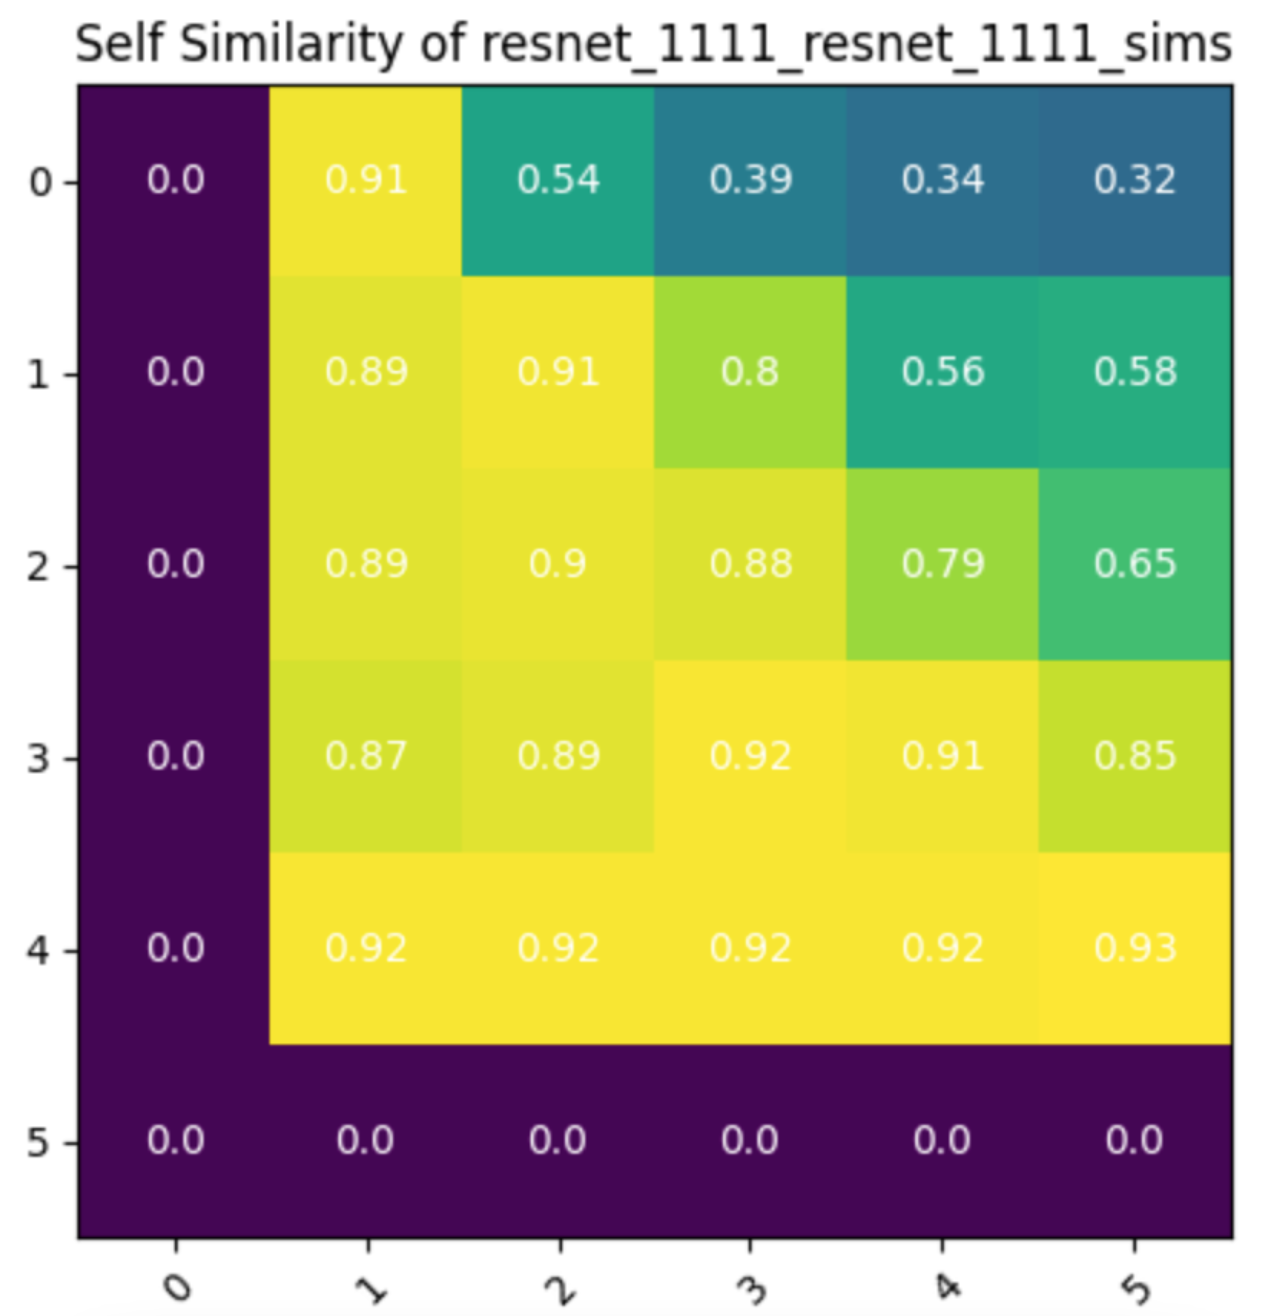
\includegraphics[width=6cm, trim={0.5cm, 2cm, 0.5cm, 2cm}, clip]{ImagePdfs/resnet1111_1111.pdf}
      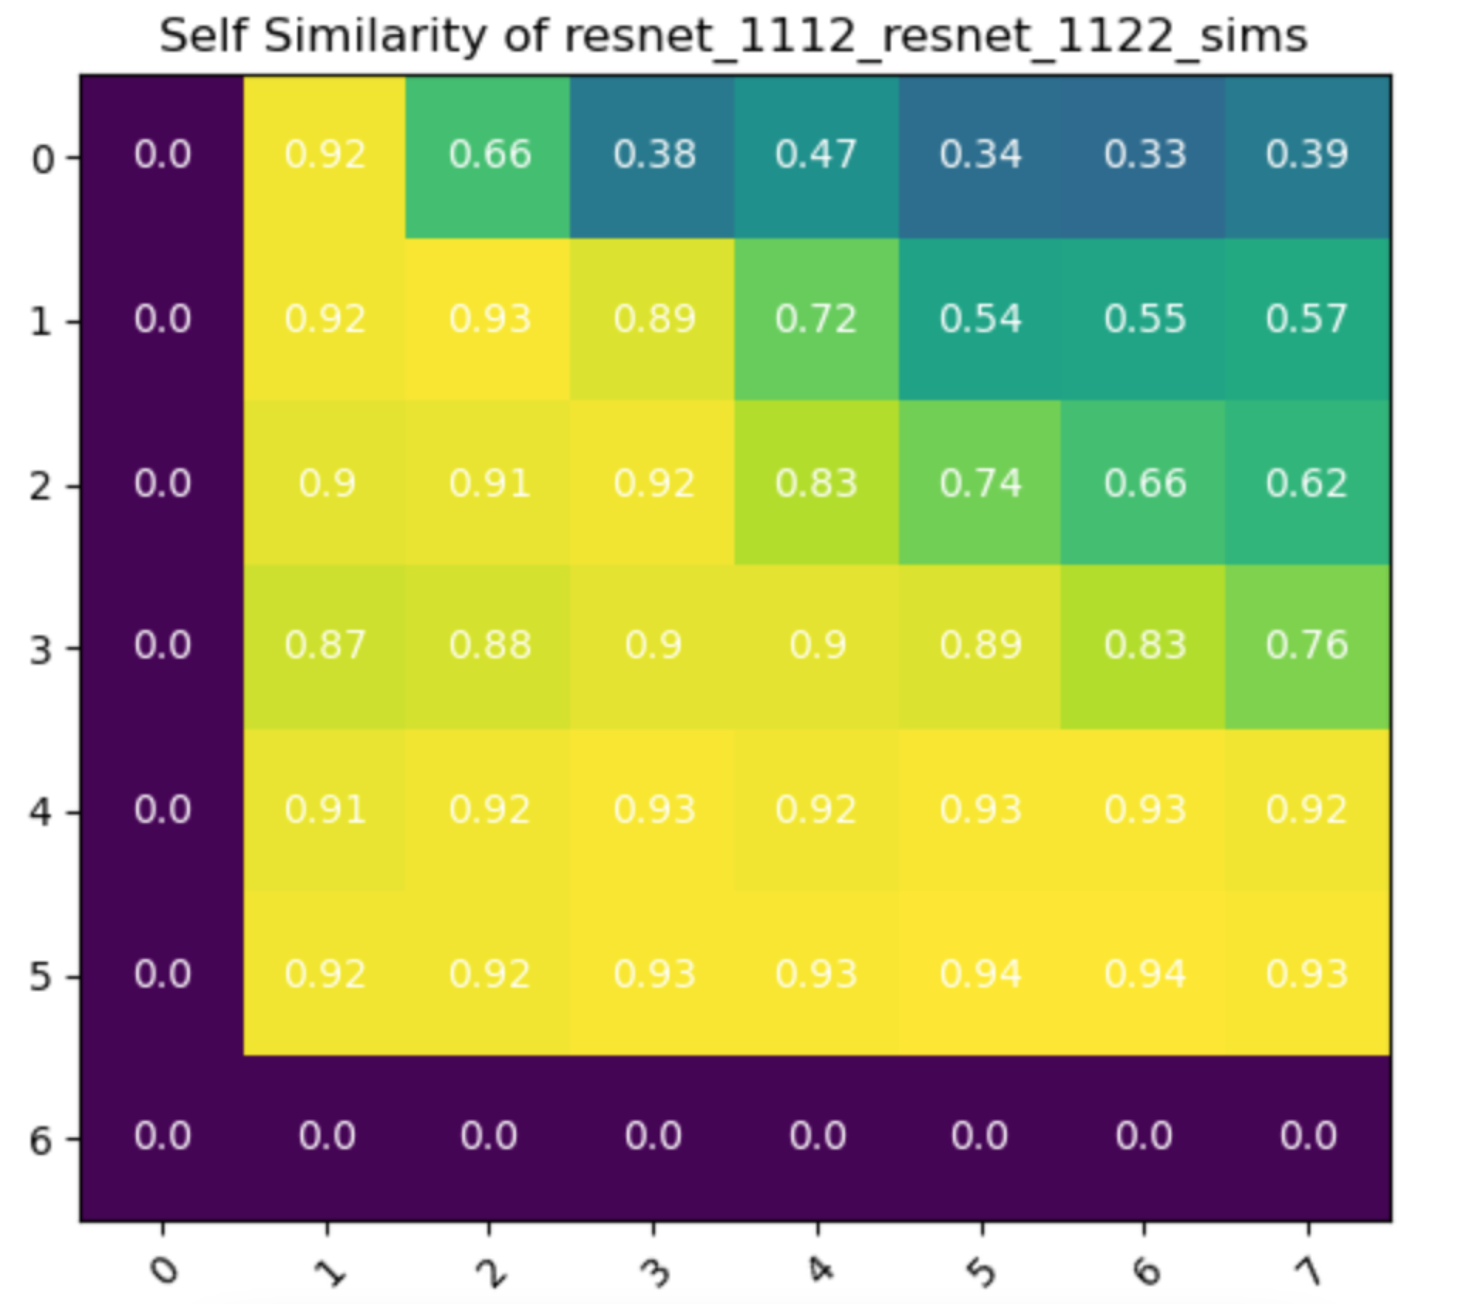
\includegraphics[width=6cm,angle=270, trim={0.25cm, 3cm, 0.25cm, 3.5cm}, clip]{ImagePdfs/resnet1112_1122.pdf}
      \caption{Triangle Pattern in Small ResNets.
      The plot is to be interpreted as a similarity matrix from sender to reciever (shifted right by one column).
      Where comparisons were not possible due to overly dissimilar shapes, a similarity of zero was logged.}
   \end{figure}
\end{center}

\label{Figure3}
\begin{center}
   \begin{figure}[H]
      \centering
      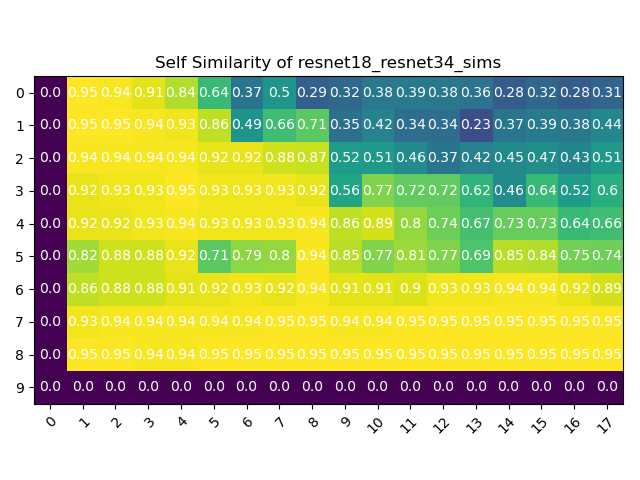
\includegraphics[width=9.5cm, trim={3cm, 7cm, 3cm, 7cm}, clip]{ImagePdfs/resnet18_resnet34_sims.pdf}
      \caption*{Triangular Pattern in Larger ResNets.
      The plot is to be interpreted, just like \hyperref[Figure2]{Figure 1} as a similarity matrix from sender to reciever
      (shifted right by one column).
      Where comparisons were not possible due to overly dissimilar shapes, a similarity of zero was logged.}
   \end{figure}
\end{center}

\label{Figure4}
\begin{center}
   \begin{figure}[H]
      \centering
      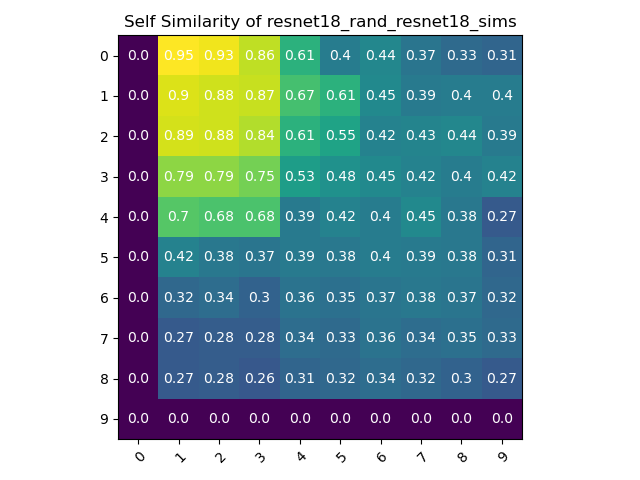
\includegraphics[width=8.5cm, trim={3cm, 7cm, 3cm, 7cm}, clip]{ImagePdfs/resnet18_rand_resnet18_sims.pdf}
      \caption*{Mostly Random (Uniform) Pattern for Random Senders. The plot is to be intrepreted, just like
      \hyperref[Figure2]{Figure 1} or \hyperref[Figure3]{Figure 2}
      as a similarity matrix from sender to reciever (shifted right by one column).
      Where comparisons were not possible due to overly dissimilar shapes, a similarity of zero was logged.}
   \end{figure}
\end{center}

\subsection*{Conclusion}
The most interesting aspect of our results is the high accuracy of the stitching network
for layers in the lower left hand triangle. Given that we interpret the stitching network accuracy
as a similarity, our results suggest that each sender representation is similar with \textit{all}
the receiver representations from a layer before it. We expected to see that each layer would be
similar to a couple (nearby) layers at most because the standard narrative has been that 
every layer loses some amount of granular information, and so that information should not be reconstructable
in a \textit{interchangeability} test like stitching.

We see two main explanations for the results. The first is that the common narrative could be wrong and some neural
networks may in fact be able to maintain most if not all of the granular information of the image throughout their
processing of it. The second is that the stitch may be able to give the reciever a representation which, despite being
different from that which is expected, nonetheless yields high accuracy.

We believe that the latter option is the most likely. Intuitively, the sttich may be able to figure out how to
generate some generic, albeit unrealistic, set of the most salient features for the recieving layer to classify
in a given way. Perhaps it is generating the ``average'' human, for example. However, a deeper analysis is required
to ascertain whether that is the case.

\newpage
\bibliography{iclr2021_conference}
\bibliographystyle{iclr2021_conference}
\end{document}
